\documentclass{book}
\usepackage[a4paper,top=2.5cm,bottom=2.5cm,left=2.5cm,right=2.5cm]{geometry}
\usepackage{makeidx}
\usepackage{natbib}
\usepackage{graphicx}
\usepackage{multicol}
\usepackage{float}
\usepackage{listings}
\usepackage{color}
\usepackage{ifthen}
\usepackage[table]{xcolor}
\usepackage{textcomp}
\usepackage{alltt}
\usepackage{ifpdf}
\ifpdf
\usepackage[pdftex,
            pagebackref=true,
            colorlinks=true,
            linkcolor=blue,
            unicode
           ]{hyperref}
\else
\usepackage[ps2pdf,
            pagebackref=true,
            colorlinks=true,
            linkcolor=blue,
            unicode
           ]{hyperref}
\usepackage{pspicture}
\fi
\usepackage[utf8]{inputenc}
\usepackage{mathptmx}
\usepackage[scaled=.90]{helvet}
\usepackage{courier}
\usepackage{sectsty}
\usepackage{amssymb}
\usepackage[titles]{tocloft}
\usepackage{doxygen}
\lstset{language=C++,inputencoding=utf8,basicstyle=\footnotesize,breaklines=true,breakatwhitespace=true,tabsize=2,numbers=left }
\makeindex
\setcounter{tocdepth}{3}
\renewcommand{\footrulewidth}{0.4pt}
\renewcommand{\familydefault}{\sfdefault}
\hfuzz=15pt
\setlength{\emergencystretch}{15pt}
\hbadness=750
\tolerance=750
\begin{document}
\hypersetup{pageanchor=false,citecolor=blue}
\begin{titlepage}
\vspace*{7cm}
\begin{center}
{\Large U\-S\-B Toolbox }\\
\vspace*{1cm}
{\large Generated by Doxygen 1.8.2}\\
\vspace*{0.5cm}
{\small Sat Oct 20 2012 10:41:23}\\
\end{center}
\end{titlepage}
\clearemptydoublepage
\pagenumbering{roman}
\tableofcontents
\clearemptydoublepage
\pagenumbering{arabic}
\hypersetup{pageanchor=true,citecolor=blue}
\chapter{Hierarchical Index}
\section{Class Hierarchy}
This inheritance list is sorted roughly, but not completely, alphabetically\-:\begin{DoxyCompactList}
\item $<$N\-S\-Application\-Delegate$>$\begin{DoxyCompactList}
\item \contentsline{section}{C\-T\-App\-Delegate}{\pageref{interface_c_t_app_delegate}}{}
\end{DoxyCompactList}
\item \contentsline{section}{N\-S\-Data(C\-T\-Data\-From\-Hex\-String)}{\pageref{category_n_s_data_07_c_t_data_from_hex_string_08}}{}
\item N\-S\-Object\begin{DoxyCompactList}
\item \contentsline{section}{C\-T\-App\-Delegate}{\pageref{interface_c_t_app_delegate}}{}
\item \contentsline{section}{C\-T\-U\-S\-B\-Device}{\pageref{interface_c_t_u_s_b_device}}{}
\end{DoxyCompactList}
\item N\-S\-Value\-Transformer\begin{DoxyCompactList}
\item \contentsline{section}{C\-T\-Number\-To\-Hex\-String\-Transformer}{\pageref{interface_c_t_number_to_hex_string_transformer}}{}
\item \contentsline{section}{C\-T\-Number\-To\-String\-Formatter}{\pageref{interface_c_t_number_to_string_formatter}}{}
\end{DoxyCompactList}
\end{DoxyCompactList}

\chapter{Class Index}
\section{Class List}
Here are the classes, structs, unions and interfaces with brief descriptions\-:\begin{DoxyCompactList}
\item\contentsline{section}{\hyperlink{interface_c_t_app_delegate}{C\-T\-App\-Delegate} }{\pageref{interface_c_t_app_delegate}}{}
\item\contentsline{section}{\hyperlink{interface_c_t_number_to_hex_string_transformer}{C\-T\-Number\-To\-Hex\-String\-Transformer} }{\pageref{interface_c_t_number_to_hex_string_transformer}}{}
\item\contentsline{section}{\hyperlink{interface_c_t_number_to_string_formatter}{C\-T\-Number\-To\-String\-Formatter} }{\pageref{interface_c_t_number_to_string_formatter}}{}
\item\contentsline{section}{\hyperlink{interface_c_t_u_s_b_device}{C\-T\-U\-S\-B\-Device} }{\pageref{interface_c_t_u_s_b_device}}{}
\item\contentsline{section}{\hyperlink{category_n_s_data_07_c_t_data_from_hex_string_08}{N\-S\-Data(\-C\-T\-Data\-From\-Hex\-String)} }{\pageref{category_n_s_data_07_c_t_data_from_hex_string_08}}{}
\end{DoxyCompactList}

\chapter{File Index}
\section{File List}
Here is a list of all files with brief descriptions\-:\begin{DoxyCompactList}
\item\contentsline{section}{U\-S\-B Toolbox/\hyperlink{_c_t_app_delegate_8h}{C\-T\-App\-Delegate.\-h} }{\pageref{_c_t_app_delegate_8h}}{}
\item\contentsline{section}{U\-S\-B Toolbox/\hyperlink{_c_t_app_delegate_8m}{C\-T\-App\-Delegate.\-m} }{\pageref{_c_t_app_delegate_8m}}{}
\item\contentsline{section}{U\-S\-B Toolbox/\hyperlink{_c_t_number_to_hex_string_transformer_8h}{C\-T\-Number\-To\-Hex\-String\-Transformer.\-h} }{\pageref{_c_t_number_to_hex_string_transformer_8h}}{}
\item\contentsline{section}{U\-S\-B Toolbox/\hyperlink{_c_t_number_to_hex_string_transformer_8m}{C\-T\-Number\-To\-Hex\-String\-Transformer.\-m} }{\pageref{_c_t_number_to_hex_string_transformer_8m}}{}
\item\contentsline{section}{U\-S\-B Toolbox/\hyperlink{_c_t_number_to_string_formatter_8h}{C\-T\-Number\-To\-String\-Formatter.\-h} }{\pageref{_c_t_number_to_string_formatter_8h}}{}
\item\contentsline{section}{U\-S\-B Toolbox/\hyperlink{_c_t_number_to_string_formatter_8m}{C\-T\-Number\-To\-String\-Formatter.\-m} }{\pageref{_c_t_number_to_string_formatter_8m}}{}
\item\contentsline{section}{U\-S\-B Toolbox/\hyperlink{main_8m}{main.\-m} }{\pageref{main_8m}}{}
\end{DoxyCompactList}

\chapter{Class Documentation}
\hypertarget{interface_c_t_app_delegate}{\section{C\-T\-App\-Delegate Class Reference}
\label{interface_c_t_app_delegate}\index{C\-T\-App\-Delegate@{C\-T\-App\-Delegate}}
}


{\ttfamily \#import $<$C\-T\-App\-Delegate.\-h$>$}

Inheritance diagram for C\-T\-App\-Delegate\-:\begin{figure}[H]
\begin{center}
\leavevmode
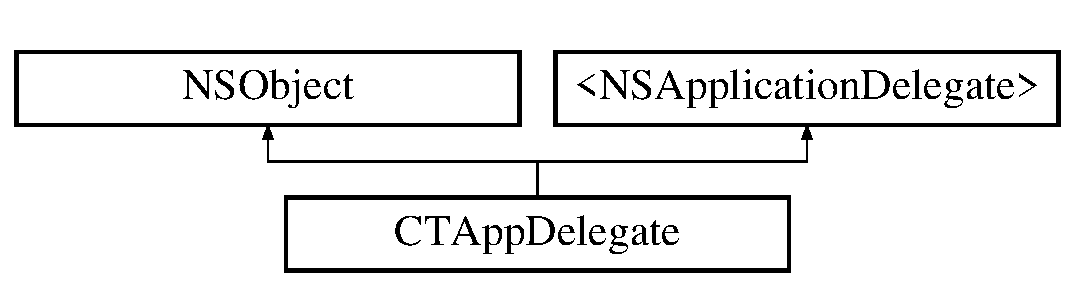
\includegraphics[height=2.000000cm]{interface_c_t_app_delegate}
\end{center}
\end{figure}
\subsection*{Instance Methods}
\begin{DoxyCompactItemize}
\item 
(void) -\/ \hyperlink{interface_c_t_app_delegate_addd3afab284b71398cf768928236ec86}{print\-String\-:}
\item 
(void) -\/ \hyperlink{interface_c_t_app_delegate_ac775ffc73129f7d3ff35305d9341a831}{print\-Data\-:length\-:}
\item 
(void) -\/ \hyperlink{interface_c_t_app_delegate_aa1ff2bd3f654a541d2790cf4ebc36386}{print\-Hex\-From\-Data\-:length\-:}
\item 
(void) -\/ \hyperlink{interface_c_t_app_delegate_adc5dedd1eee0e8b1fc126764f1f242dd}{print\-Plain\-Text\-From\-Data\-:length\-:}
\item 
(void) -\/ \hyperlink{interface_c_t_app_delegate_ae7974427860f64ab0225f32237b11179}{print\-Lib\-U\-S\-B\-Error\-:with\-Operation\-:}
\item 
(N\-S\-Data $\ast$) -\/ \hyperlink{interface_c_t_app_delegate_ae71bc249cd087494e9b00e49988b5b55}{data\-From\-Hex\-String\-:}
\begin{DoxyCompactList}\small\item\em Convers a hex formatted N\-S\-String to N\-S\-Data. \end{DoxyCompactList}\item 
(I\-B\-Action) -\/ \hyperlink{interface_c_t_app_delegate_a0061d4cbac40771a21e02323bedbf32b}{do\-Bulk\-Transfer\-:}
\item 
(I\-B\-Action) -\/ \hyperlink{interface_c_t_app_delegate_a477526454468a7a90dd85aaffad30a57}{do\-U\-S\-B\-Control\-Transfer\-:}
\item 
(I\-B\-Action) -\/ \hyperlink{interface_c_t_app_delegate_a21bf37f0abad2c4ba4728db09b3eb6e5}{list\-All\-Attached\-U\-S\-B\-Devices\-:}
\item 
(I\-B\-Action) -\/ \hyperlink{interface_c_t_app_delegate_ae6fb4f8759991c57bfdd0eb1c89821e3}{clear\-Console\-:}
\item 
(U\-Int8) -\/ \hyperlink{interface_c_t_app_delegate_a8e6db21c4bf9f1813527f4951572b3c8}{convert\-N\-S\-String\-To\-U\-Int8}
\item 
(U\-Int16) -\/ \hyperlink{interface_c_t_app_delegate_ae19f27002aa800030e0fa74b2d6b5237}{convert\-N\-S\-String\-To\-U\-Int16}
\end{DoxyCompactItemize}
\subsection*{Protected Attributes}
\begin{DoxyCompactItemize}
\item 
I\-B\-Outlet N\-S\-Window $\ast$ \hyperlink{interface_c_t_app_delegate_a0e5d80a8d3d78945c2b14d477a71c0eb}{main\-Window}
\item 
I\-B\-Outlet N\-S\-Text\-View $\ast$ \hyperlink{interface_c_t_app_delegate_a02680c24bf116eb7869cfe0489b2a381}{console\-Text\-View}
\item 
I\-B\-Outlet N\-S\-Text\-View $\ast$ \hyperlink{interface_c_t_app_delegate_abf8e0f79b36a4b23262ba2a2d29eabe7}{input\-Text\-View}
\item 
I\-B\-Outlet N\-S\-User\-Defaults\-Controller $\ast$ \hyperlink{interface_c_t_app_delegate_a55373d5265a108cb12510bd086aa15e8}{user\-Defaults\-Controller}
\item 
libusb\-\_\-device $\ast$$\ast$ \hyperlink{interface_c_t_app_delegate_a9d80eb0a8fb6f9c373648cba3dbe5b26}{all\-U\-S\-B\-Devices}
\item 
libusb\-\_\-device\-\_\-handle $\ast$ \hyperlink{interface_c_t_app_delegate_a0efa5af44bc03361f0953b7946461635}{U\-S\-B\-Device\-Handle}
\item 
libusb\-\_\-device $\ast$ \hyperlink{interface_c_t_app_delegate_ac20589aa72af723c196a1251c22fc093}{the\-U\-S\-B\-Device}
\item 
ssize\-\_\-t \hyperlink{interface_c_t_app_delegate_aab4901a3d0ce6c86771365bbf1645eeb}{number\-Of\-U\-S\-B\-Devices}
\item 
N\-S\-Mutable\-Attributed\-String $\ast$ \hyperlink{interface_c_t_app_delegate_a46c927de3b01529297fa0e078e486f19}{output\-Text\-Storage}
\item 
N\-S\-Mutable\-Attributed\-String $\ast$ \hyperlink{interface_c_t_app_delegate_a267286c82789444b42d30238c62b38bc}{input\-Text\-Storage}
\end{DoxyCompactItemize}
\subsection*{Properties}
\begin{DoxyCompactItemize}
\item 
N\-S\-Color $\ast$ \hyperlink{interface_c_t_app_delegate_ab0bb80237b8aa297ec48dec224eddbb7}{console\-Error\-Text\-Color}
\item 
N\-S\-Color $\ast$ \hyperlink{interface_c_t_app_delegate_a5b184ad30f043f8eb642ef9f21f11555}{console\-Information\-Text\-Color}
\item 
N\-S\-Color $\ast$ \hyperlink{interface_c_t_app_delegate_a51aebba711d81a108659db7f5a2e3509}{console\-Data\-Text\-Color}
\item 
N\-S\-Color $\ast$ \hyperlink{interface_c_t_app_delegate_a9fc48b94e012554988d71fab9fc854b8}{console\-Background\-Color}
\item 
N\-S\-Number $\ast$ \hyperlink{interface_c_t_app_delegate_a4578b9f0c04d7376bde881085bad233a}{display\-Hex\-Or\-Plain\-Text}
\item 
N\-S\-Number $\ast$ \hyperlink{interface_c_t_app_delegate_ae808b0548069c03cc1912db1c83891eb}{bulk\-Transfer\-Endpoint}
\item 
N\-S\-Number $\ast$ \hyperlink{interface_c_t_app_delegate_adea2205a53bdecd999d70b5abd08696f}{bulk\-Transfer\-Direction}
\item 
N\-S\-Number $\ast$ \hyperlink{interface_c_t_app_delegate_ac4efbc9d53180254895b9733fe3d376e}{bulk\-Transfer\-Length}
\item 
N\-S\-Number $\ast$ \hyperlink{interface_c_t_app_delegate_ac3f78415dd122de7cebf7a3745a69da9}{device\-V\-I\-D}
\item 
N\-S\-Number $\ast$ \hyperlink{interface_c_t_app_delegate_a5803369bf1901ee34be36dbdd3eb3734}{device\-P\-I\-D}
\item 
N\-S\-Number $\ast$ \hyperlink{interface_c_t_app_delegate_ae0366c6888903dc8247ecf1f2dacc69d}{request\-Type}
\item 
N\-S\-Number $\ast$ \hyperlink{interface_c_t_app_delegate_a91630675dd1cdd1844fdd217ce52bf86}{request\-Destination}
\item 
N\-S\-Number $\ast$ \hyperlink{interface_c_t_app_delegate_aade0217b509c082080b919e7a9f55046}{control\-Transfer\-Request}
\item 
N\-S\-Number $\ast$ \hyperlink{interface_c_t_app_delegate_a62fe8f350142e22ead502a51f201cb1f}{control\-Transfer\-Value}
\item 
N\-S\-Number $\ast$ \hyperlink{interface_c_t_app_delegate_af08e59f3a506606bfa91e079b9ae16a6}{control\-Transfer\-Index}
\item 
N\-S\-Number $\ast$ \hyperlink{interface_c_t_app_delegate_afb1667e9e2db3e2b289a099508a338d5}{control\-Transfer\-Length}
\end{DoxyCompactItemize}


\subsection{Method Documentation}
\hypertarget{interface_c_t_app_delegate_ae6fb4f8759991c57bfdd0eb1c89821e3}{\index{C\-T\-App\-Delegate@{C\-T\-App\-Delegate}!clear\-Console\-:@{clear\-Console\-:}}
\index{clear\-Console\-:@{clear\-Console\-:}!CTAppDelegate@{C\-T\-App\-Delegate}}
\subsubsection[{clear\-Console\-:}]{\setlength{\rightskip}{0pt plus 5cm}-\/ (I\-B\-Action) clear\-Console\-: 
\begin{DoxyParamCaption}
\item[{(id)}]{sender}
\end{DoxyParamCaption}
}}\label{interface_c_t_app_delegate_ae6fb4f8759991c57bfdd0eb1c89821e3}
\hypertarget{interface_c_t_app_delegate_ae19f27002aa800030e0fa74b2d6b5237}{\index{C\-T\-App\-Delegate@{C\-T\-App\-Delegate}!convert\-N\-S\-String\-To\-U\-Int16@{convert\-N\-S\-String\-To\-U\-Int16}}
\index{convert\-N\-S\-String\-To\-U\-Int16@{convert\-N\-S\-String\-To\-U\-Int16}!CTAppDelegate@{C\-T\-App\-Delegate}}
\subsubsection[{convert\-N\-S\-String\-To\-U\-Int16}]{\setlength{\rightskip}{0pt plus 5cm}-\/ (U\-Int16) convert\-N\-S\-String\-To\-U\-Int16 
\begin{DoxyParamCaption}
\item[{(N\-S\-String $\ast$)}]{the\-String}
\end{DoxyParamCaption}
}}\label{interface_c_t_app_delegate_ae19f27002aa800030e0fa74b2d6b5237}
\hypertarget{interface_c_t_app_delegate_a8e6db21c4bf9f1813527f4951572b3c8}{\index{C\-T\-App\-Delegate@{C\-T\-App\-Delegate}!convert\-N\-S\-String\-To\-U\-Int8@{convert\-N\-S\-String\-To\-U\-Int8}}
\index{convert\-N\-S\-String\-To\-U\-Int8@{convert\-N\-S\-String\-To\-U\-Int8}!CTAppDelegate@{C\-T\-App\-Delegate}}
\subsubsection[{convert\-N\-S\-String\-To\-U\-Int8}]{\setlength{\rightskip}{0pt plus 5cm}-\/ (U\-Int8) convert\-N\-S\-String\-To\-U\-Int8 
\begin{DoxyParamCaption}
\item[{(N\-S\-String $\ast$)}]{the\-String}
\end{DoxyParamCaption}
}}\label{interface_c_t_app_delegate_a8e6db21c4bf9f1813527f4951572b3c8}
\hypertarget{interface_c_t_app_delegate_ae71bc249cd087494e9b00e49988b5b55}{\index{C\-T\-App\-Delegate@{C\-T\-App\-Delegate}!data\-From\-Hex\-String\-:@{data\-From\-Hex\-String\-:}}
\index{data\-From\-Hex\-String\-:@{data\-From\-Hex\-String\-:}!CTAppDelegate@{C\-T\-App\-Delegate}}
\subsubsection[{data\-From\-Hex\-String\-:}]{\setlength{\rightskip}{0pt plus 5cm}-\/ (N\-S\-Data $\ast$) data\-From\-Hex\-String\-: 
\begin{DoxyParamCaption}
\item[{(N\-S\-String $\ast$)}]{the\-String}
\end{DoxyParamCaption}
}}\label{interface_c_t_app_delegate_ae71bc249cd087494e9b00e49988b5b55}


Convers a hex formatted N\-S\-String to N\-S\-Data. 


\begin{DoxyParams}{Parameters}
{\em the\-String} & \\
\hline
\end{DoxyParams}
\begin{DoxyReturn}{Returns}
N\-S\-Data 
\end{DoxyReturn}

\begin{DoxyExceptions}{Exceptions}
{\em none} & \\
\hline
\end{DoxyExceptions}
\hypertarget{interface_c_t_app_delegate_a0061d4cbac40771a21e02323bedbf32b}{\index{C\-T\-App\-Delegate@{C\-T\-App\-Delegate}!do\-Bulk\-Transfer\-:@{do\-Bulk\-Transfer\-:}}
\index{do\-Bulk\-Transfer\-:@{do\-Bulk\-Transfer\-:}!CTAppDelegate@{C\-T\-App\-Delegate}}
\subsubsection[{do\-Bulk\-Transfer\-:}]{\setlength{\rightskip}{0pt plus 5cm}-\/ (I\-B\-Action) do\-Bulk\-Transfer\-: 
\begin{DoxyParamCaption}
\item[{(id)}]{sender}
\end{DoxyParamCaption}
}}\label{interface_c_t_app_delegate_a0061d4cbac40771a21e02323bedbf32b}
\hypertarget{interface_c_t_app_delegate_a477526454468a7a90dd85aaffad30a57}{\index{C\-T\-App\-Delegate@{C\-T\-App\-Delegate}!do\-U\-S\-B\-Control\-Transfer\-:@{do\-U\-S\-B\-Control\-Transfer\-:}}
\index{do\-U\-S\-B\-Control\-Transfer\-:@{do\-U\-S\-B\-Control\-Transfer\-:}!CTAppDelegate@{C\-T\-App\-Delegate}}
\subsubsection[{do\-U\-S\-B\-Control\-Transfer\-:}]{\setlength{\rightskip}{0pt plus 5cm}-\/ (I\-B\-Action) do\-U\-S\-B\-Control\-Transfer\-: 
\begin{DoxyParamCaption}
\item[{(id)}]{sender}
\end{DoxyParamCaption}
}}\label{interface_c_t_app_delegate_a477526454468a7a90dd85aaffad30a57}
\hypertarget{interface_c_t_app_delegate_a21bf37f0abad2c4ba4728db09b3eb6e5}{\index{C\-T\-App\-Delegate@{C\-T\-App\-Delegate}!list\-All\-Attached\-U\-S\-B\-Devices\-:@{list\-All\-Attached\-U\-S\-B\-Devices\-:}}
\index{list\-All\-Attached\-U\-S\-B\-Devices\-:@{list\-All\-Attached\-U\-S\-B\-Devices\-:}!CTAppDelegate@{C\-T\-App\-Delegate}}
\subsubsection[{list\-All\-Attached\-U\-S\-B\-Devices\-:}]{\setlength{\rightskip}{0pt plus 5cm}-\/ (I\-B\-Action) list\-All\-Attached\-U\-S\-B\-Devices\-: 
\begin{DoxyParamCaption}
\item[{(id)}]{sender}
\end{DoxyParamCaption}
}}\label{interface_c_t_app_delegate_a21bf37f0abad2c4ba4728db09b3eb6e5}
\hypertarget{interface_c_t_app_delegate_ac775ffc73129f7d3ff35305d9341a831}{\index{C\-T\-App\-Delegate@{C\-T\-App\-Delegate}!print\-Data\-:length\-:@{print\-Data\-:length\-:}}
\index{print\-Data\-:length\-:@{print\-Data\-:length\-:}!CTAppDelegate@{C\-T\-App\-Delegate}}
\subsubsection[{print\-Data\-:length\-:}]{\setlength{\rightskip}{0pt plus 5cm}-\/ (void) print\-Data\-: 
\begin{DoxyParamCaption}
\item[{(unsigned char $\ast$)}]{the\-Data}
\item[{length:(int)}]{the\-Length}
\end{DoxyParamCaption}
}}\label{interface_c_t_app_delegate_ac775ffc73129f7d3ff35305d9341a831}
\hypertarget{interface_c_t_app_delegate_aa1ff2bd3f654a541d2790cf4ebc36386}{\index{C\-T\-App\-Delegate@{C\-T\-App\-Delegate}!print\-Hex\-From\-Data\-:length\-:@{print\-Hex\-From\-Data\-:length\-:}}
\index{print\-Hex\-From\-Data\-:length\-:@{print\-Hex\-From\-Data\-:length\-:}!CTAppDelegate@{C\-T\-App\-Delegate}}
\subsubsection[{print\-Hex\-From\-Data\-:length\-:}]{\setlength{\rightskip}{0pt plus 5cm}-\/ (void) print\-Hex\-From\-Data\-: 
\begin{DoxyParamCaption}
\item[{(unsigned char $\ast$)}]{the\-Data}
\item[{length:(int)}]{the\-Length}
\end{DoxyParamCaption}
}}\label{interface_c_t_app_delegate_aa1ff2bd3f654a541d2790cf4ebc36386}
\hypertarget{interface_c_t_app_delegate_ae7974427860f64ab0225f32237b11179}{\index{C\-T\-App\-Delegate@{C\-T\-App\-Delegate}!print\-Lib\-U\-S\-B\-Error\-:with\-Operation\-:@{print\-Lib\-U\-S\-B\-Error\-:with\-Operation\-:}}
\index{print\-Lib\-U\-S\-B\-Error\-:with\-Operation\-:@{print\-Lib\-U\-S\-B\-Error\-:with\-Operation\-:}!CTAppDelegate@{C\-T\-App\-Delegate}}
\subsubsection[{print\-Lib\-U\-S\-B\-Error\-:with\-Operation\-:}]{\setlength{\rightskip}{0pt plus 5cm}-\/ (void) print\-Lib\-U\-S\-B\-Error\-: 
\begin{DoxyParamCaption}
\item[{(int)}]{the\-Error}
\item[{withOperation:(N\-S\-String $\ast$)}]{the\-Operation}
\end{DoxyParamCaption}
}}\label{interface_c_t_app_delegate_ae7974427860f64ab0225f32237b11179}
\hypertarget{interface_c_t_app_delegate_adc5dedd1eee0e8b1fc126764f1f242dd}{\index{C\-T\-App\-Delegate@{C\-T\-App\-Delegate}!print\-Plain\-Text\-From\-Data\-:length\-:@{print\-Plain\-Text\-From\-Data\-:length\-:}}
\index{print\-Plain\-Text\-From\-Data\-:length\-:@{print\-Plain\-Text\-From\-Data\-:length\-:}!CTAppDelegate@{C\-T\-App\-Delegate}}
\subsubsection[{print\-Plain\-Text\-From\-Data\-:length\-:}]{\setlength{\rightskip}{0pt plus 5cm}-\/ (void) print\-Plain\-Text\-From\-Data\-: 
\begin{DoxyParamCaption}
\item[{(unsigned char $\ast$)}]{the\-Data}
\item[{length:(int)}]{the\-Length}
\end{DoxyParamCaption}
}}\label{interface_c_t_app_delegate_adc5dedd1eee0e8b1fc126764f1f242dd}
\hypertarget{interface_c_t_app_delegate_addd3afab284b71398cf768928236ec86}{\index{C\-T\-App\-Delegate@{C\-T\-App\-Delegate}!print\-String\-:@{print\-String\-:}}
\index{print\-String\-:@{print\-String\-:}!CTAppDelegate@{C\-T\-App\-Delegate}}
\subsubsection[{print\-String\-:}]{\setlength{\rightskip}{0pt plus 5cm}-\/ (void) print\-String\-: 
\begin{DoxyParamCaption}
\item[{(N\-S\-String $\ast$)}]{the\-String}
\end{DoxyParamCaption}
}}\label{interface_c_t_app_delegate_addd3afab284b71398cf768928236ec86}


\subsection{Member Data Documentation}
\hypertarget{interface_c_t_app_delegate_a9d80eb0a8fb6f9c373648cba3dbe5b26}{\index{C\-T\-App\-Delegate@{C\-T\-App\-Delegate}!all\-U\-S\-B\-Devices@{all\-U\-S\-B\-Devices}}
\index{all\-U\-S\-B\-Devices@{all\-U\-S\-B\-Devices}!CTAppDelegate@{C\-T\-App\-Delegate}}
\subsubsection[{all\-U\-S\-B\-Devices}]{\setlength{\rightskip}{0pt plus 5cm}-\/ (libusb\-\_\-device$\ast$$\ast$) all\-U\-S\-B\-Devices\hspace{0.3cm}{\ttfamily [protected]}}}\label{interface_c_t_app_delegate_a9d80eb0a8fb6f9c373648cba3dbe5b26}
\hypertarget{interface_c_t_app_delegate_a02680c24bf116eb7869cfe0489b2a381}{\index{C\-T\-App\-Delegate@{C\-T\-App\-Delegate}!console\-Text\-View@{console\-Text\-View}}
\index{console\-Text\-View@{console\-Text\-View}!CTAppDelegate@{C\-T\-App\-Delegate}}
\subsubsection[{console\-Text\-View}]{\setlength{\rightskip}{0pt plus 5cm}-\/ (I\-B\-Outlet N\-S\-Text\-View$\ast$) console\-Text\-View\hspace{0.3cm}{\ttfamily [protected]}}}\label{interface_c_t_app_delegate_a02680c24bf116eb7869cfe0489b2a381}
\hypertarget{interface_c_t_app_delegate_a267286c82789444b42d30238c62b38bc}{\index{C\-T\-App\-Delegate@{C\-T\-App\-Delegate}!input\-Text\-Storage@{input\-Text\-Storage}}
\index{input\-Text\-Storage@{input\-Text\-Storage}!CTAppDelegate@{C\-T\-App\-Delegate}}
\subsubsection[{input\-Text\-Storage}]{\setlength{\rightskip}{0pt plus 5cm}-\/ (N\-S\-Mutable\-Attributed\-String$\ast$) input\-Text\-Storage\hspace{0.3cm}{\ttfamily [protected]}}}\label{interface_c_t_app_delegate_a267286c82789444b42d30238c62b38bc}
\hypertarget{interface_c_t_app_delegate_abf8e0f79b36a4b23262ba2a2d29eabe7}{\index{C\-T\-App\-Delegate@{C\-T\-App\-Delegate}!input\-Text\-View@{input\-Text\-View}}
\index{input\-Text\-View@{input\-Text\-View}!CTAppDelegate@{C\-T\-App\-Delegate}}
\subsubsection[{input\-Text\-View}]{\setlength{\rightskip}{0pt plus 5cm}-\/ (I\-B\-Outlet N\-S\-Text\-View$\ast$) input\-Text\-View\hspace{0.3cm}{\ttfamily [protected]}}}\label{interface_c_t_app_delegate_abf8e0f79b36a4b23262ba2a2d29eabe7}
\hypertarget{interface_c_t_app_delegate_a0e5d80a8d3d78945c2b14d477a71c0eb}{\index{C\-T\-App\-Delegate@{C\-T\-App\-Delegate}!main\-Window@{main\-Window}}
\index{main\-Window@{main\-Window}!CTAppDelegate@{C\-T\-App\-Delegate}}
\subsubsection[{main\-Window}]{\setlength{\rightskip}{0pt plus 5cm}-\/ (I\-B\-Outlet N\-S\-Window$\ast$) main\-Window\hspace{0.3cm}{\ttfamily [protected]}}}\label{interface_c_t_app_delegate_a0e5d80a8d3d78945c2b14d477a71c0eb}
\hypertarget{interface_c_t_app_delegate_aab4901a3d0ce6c86771365bbf1645eeb}{\index{C\-T\-App\-Delegate@{C\-T\-App\-Delegate}!number\-Of\-U\-S\-B\-Devices@{number\-Of\-U\-S\-B\-Devices}}
\index{number\-Of\-U\-S\-B\-Devices@{number\-Of\-U\-S\-B\-Devices}!CTAppDelegate@{C\-T\-App\-Delegate}}
\subsubsection[{number\-Of\-U\-S\-B\-Devices}]{\setlength{\rightskip}{0pt plus 5cm}-\/ (ssize\-\_\-t) number\-Of\-U\-S\-B\-Devices\hspace{0.3cm}{\ttfamily [protected]}}}\label{interface_c_t_app_delegate_aab4901a3d0ce6c86771365bbf1645eeb}
\hypertarget{interface_c_t_app_delegate_a46c927de3b01529297fa0e078e486f19}{\index{C\-T\-App\-Delegate@{C\-T\-App\-Delegate}!output\-Text\-Storage@{output\-Text\-Storage}}
\index{output\-Text\-Storage@{output\-Text\-Storage}!CTAppDelegate@{C\-T\-App\-Delegate}}
\subsubsection[{output\-Text\-Storage}]{\setlength{\rightskip}{0pt plus 5cm}-\/ (N\-S\-Mutable\-Attributed\-String$\ast$) output\-Text\-Storage\hspace{0.3cm}{\ttfamily [protected]}}}\label{interface_c_t_app_delegate_a46c927de3b01529297fa0e078e486f19}
\hypertarget{interface_c_t_app_delegate_ac20589aa72af723c196a1251c22fc093}{\index{C\-T\-App\-Delegate@{C\-T\-App\-Delegate}!the\-U\-S\-B\-Device@{the\-U\-S\-B\-Device}}
\index{the\-U\-S\-B\-Device@{the\-U\-S\-B\-Device}!CTAppDelegate@{C\-T\-App\-Delegate}}
\subsubsection[{the\-U\-S\-B\-Device}]{\setlength{\rightskip}{0pt plus 5cm}-\/ (libusb\-\_\-device$\ast$) the\-U\-S\-B\-Device\hspace{0.3cm}{\ttfamily [protected]}}}\label{interface_c_t_app_delegate_ac20589aa72af723c196a1251c22fc093}
\hypertarget{interface_c_t_app_delegate_a0efa5af44bc03361f0953b7946461635}{\index{C\-T\-App\-Delegate@{C\-T\-App\-Delegate}!U\-S\-B\-Device\-Handle@{U\-S\-B\-Device\-Handle}}
\index{U\-S\-B\-Device\-Handle@{U\-S\-B\-Device\-Handle}!CTAppDelegate@{C\-T\-App\-Delegate}}
\subsubsection[{U\-S\-B\-Device\-Handle}]{\setlength{\rightskip}{0pt plus 5cm}-\/ (libusb\-\_\-device\-\_\-handle$\ast$) U\-S\-B\-Device\-Handle\hspace{0.3cm}{\ttfamily [protected]}}}\label{interface_c_t_app_delegate_a0efa5af44bc03361f0953b7946461635}
\hypertarget{interface_c_t_app_delegate_a55373d5265a108cb12510bd086aa15e8}{\index{C\-T\-App\-Delegate@{C\-T\-App\-Delegate}!user\-Defaults\-Controller@{user\-Defaults\-Controller}}
\index{user\-Defaults\-Controller@{user\-Defaults\-Controller}!CTAppDelegate@{C\-T\-App\-Delegate}}
\subsubsection[{user\-Defaults\-Controller}]{\setlength{\rightskip}{0pt plus 5cm}-\/ (I\-B\-Outlet N\-S\-User\-Defaults\-Controller$\ast$) user\-Defaults\-Controller\hspace{0.3cm}{\ttfamily [protected]}}}\label{interface_c_t_app_delegate_a55373d5265a108cb12510bd086aa15e8}


\subsection{Property Documentation}
\hypertarget{interface_c_t_app_delegate_adea2205a53bdecd999d70b5abd08696f}{\index{C\-T\-App\-Delegate@{C\-T\-App\-Delegate}!bulk\-Transfer\-Direction@{bulk\-Transfer\-Direction}}
\index{bulk\-Transfer\-Direction@{bulk\-Transfer\-Direction}!CTAppDelegate@{C\-T\-App\-Delegate}}
\subsubsection[{bulk\-Transfer\-Direction}]{\setlength{\rightskip}{0pt plus 5cm}-\/ (N\-S\-Number$\ast$) bulk\-Transfer\-Direction\hspace{0.3cm}{\ttfamily [read]}, {\ttfamily [write]}, {\ttfamily [atomic]}, {\ttfamily [copy]}}}\label{interface_c_t_app_delegate_adea2205a53bdecd999d70b5abd08696f}
\hypertarget{interface_c_t_app_delegate_ae808b0548069c03cc1912db1c83891eb}{\index{C\-T\-App\-Delegate@{C\-T\-App\-Delegate}!bulk\-Transfer\-Endpoint@{bulk\-Transfer\-Endpoint}}
\index{bulk\-Transfer\-Endpoint@{bulk\-Transfer\-Endpoint}!CTAppDelegate@{C\-T\-App\-Delegate}}
\subsubsection[{bulk\-Transfer\-Endpoint}]{\setlength{\rightskip}{0pt plus 5cm}-\/ (N\-S\-Number$\ast$) bulk\-Transfer\-Endpoint\hspace{0.3cm}{\ttfamily [read]}, {\ttfamily [write]}, {\ttfamily [atomic]}, {\ttfamily [copy]}}}\label{interface_c_t_app_delegate_ae808b0548069c03cc1912db1c83891eb}
\hypertarget{interface_c_t_app_delegate_ac4efbc9d53180254895b9733fe3d376e}{\index{C\-T\-App\-Delegate@{C\-T\-App\-Delegate}!bulk\-Transfer\-Length@{bulk\-Transfer\-Length}}
\index{bulk\-Transfer\-Length@{bulk\-Transfer\-Length}!CTAppDelegate@{C\-T\-App\-Delegate}}
\subsubsection[{bulk\-Transfer\-Length}]{\setlength{\rightskip}{0pt plus 5cm}-\/ (N\-S\-Number$\ast$) bulk\-Transfer\-Length\hspace{0.3cm}{\ttfamily [read]}, {\ttfamily [write]}, {\ttfamily [atomic]}, {\ttfamily [copy]}}}\label{interface_c_t_app_delegate_ac4efbc9d53180254895b9733fe3d376e}
\hypertarget{interface_c_t_app_delegate_a9fc48b94e012554988d71fab9fc854b8}{\index{C\-T\-App\-Delegate@{C\-T\-App\-Delegate}!console\-Background\-Color@{console\-Background\-Color}}
\index{console\-Background\-Color@{console\-Background\-Color}!CTAppDelegate@{C\-T\-App\-Delegate}}
\subsubsection[{console\-Background\-Color}]{\setlength{\rightskip}{0pt plus 5cm}-\/ (N\-S\-Color$\ast$) console\-Background\-Color\hspace{0.3cm}{\ttfamily [read]}, {\ttfamily [write]}, {\ttfamily [atomic]}, {\ttfamily [copy]}}}\label{interface_c_t_app_delegate_a9fc48b94e012554988d71fab9fc854b8}
\hypertarget{interface_c_t_app_delegate_a51aebba711d81a108659db7f5a2e3509}{\index{C\-T\-App\-Delegate@{C\-T\-App\-Delegate}!console\-Data\-Text\-Color@{console\-Data\-Text\-Color}}
\index{console\-Data\-Text\-Color@{console\-Data\-Text\-Color}!CTAppDelegate@{C\-T\-App\-Delegate}}
\subsubsection[{console\-Data\-Text\-Color}]{\setlength{\rightskip}{0pt plus 5cm}-\/ (N\-S\-Color$\ast$) console\-Data\-Text\-Color\hspace{0.3cm}{\ttfamily [read]}, {\ttfamily [write]}, {\ttfamily [atomic]}, {\ttfamily [copy]}}}\label{interface_c_t_app_delegate_a51aebba711d81a108659db7f5a2e3509}
\hypertarget{interface_c_t_app_delegate_ab0bb80237b8aa297ec48dec224eddbb7}{\index{C\-T\-App\-Delegate@{C\-T\-App\-Delegate}!console\-Error\-Text\-Color@{console\-Error\-Text\-Color}}
\index{console\-Error\-Text\-Color@{console\-Error\-Text\-Color}!CTAppDelegate@{C\-T\-App\-Delegate}}
\subsubsection[{console\-Error\-Text\-Color}]{\setlength{\rightskip}{0pt plus 5cm}-\/ (N\-S\-Color$\ast$) console\-Error\-Text\-Color\hspace{0.3cm}{\ttfamily [read]}, {\ttfamily [write]}, {\ttfamily [atomic]}, {\ttfamily [copy]}}}\label{interface_c_t_app_delegate_ab0bb80237b8aa297ec48dec224eddbb7}
\hypertarget{interface_c_t_app_delegate_a5b184ad30f043f8eb642ef9f21f11555}{\index{C\-T\-App\-Delegate@{C\-T\-App\-Delegate}!console\-Information\-Text\-Color@{console\-Information\-Text\-Color}}
\index{console\-Information\-Text\-Color@{console\-Information\-Text\-Color}!CTAppDelegate@{C\-T\-App\-Delegate}}
\subsubsection[{console\-Information\-Text\-Color}]{\setlength{\rightskip}{0pt plus 5cm}-\/ (N\-S\-Color$\ast$) console\-Information\-Text\-Color\hspace{0.3cm}{\ttfamily [read]}, {\ttfamily [write]}, {\ttfamily [atomic]}, {\ttfamily [copy]}}}\label{interface_c_t_app_delegate_a5b184ad30f043f8eb642ef9f21f11555}
\hypertarget{interface_c_t_app_delegate_af08e59f3a506606bfa91e079b9ae16a6}{\index{C\-T\-App\-Delegate@{C\-T\-App\-Delegate}!control\-Transfer\-Index@{control\-Transfer\-Index}}
\index{control\-Transfer\-Index@{control\-Transfer\-Index}!CTAppDelegate@{C\-T\-App\-Delegate}}
\subsubsection[{control\-Transfer\-Index}]{\setlength{\rightskip}{0pt plus 5cm}-\/ (N\-S\-Number$\ast$) control\-Transfer\-Index\hspace{0.3cm}{\ttfamily [read]}, {\ttfamily [write]}, {\ttfamily [atomic]}, {\ttfamily [copy]}}}\label{interface_c_t_app_delegate_af08e59f3a506606bfa91e079b9ae16a6}
\hypertarget{interface_c_t_app_delegate_afb1667e9e2db3e2b289a099508a338d5}{\index{C\-T\-App\-Delegate@{C\-T\-App\-Delegate}!control\-Transfer\-Length@{control\-Transfer\-Length}}
\index{control\-Transfer\-Length@{control\-Transfer\-Length}!CTAppDelegate@{C\-T\-App\-Delegate}}
\subsubsection[{control\-Transfer\-Length}]{\setlength{\rightskip}{0pt plus 5cm}-\/ (N\-S\-Number$\ast$) control\-Transfer\-Length\hspace{0.3cm}{\ttfamily [read]}, {\ttfamily [write]}, {\ttfamily [atomic]}, {\ttfamily [copy]}}}\label{interface_c_t_app_delegate_afb1667e9e2db3e2b289a099508a338d5}
\hypertarget{interface_c_t_app_delegate_aade0217b509c082080b919e7a9f55046}{\index{C\-T\-App\-Delegate@{C\-T\-App\-Delegate}!control\-Transfer\-Request@{control\-Transfer\-Request}}
\index{control\-Transfer\-Request@{control\-Transfer\-Request}!CTAppDelegate@{C\-T\-App\-Delegate}}
\subsubsection[{control\-Transfer\-Request}]{\setlength{\rightskip}{0pt plus 5cm}-\/ (N\-S\-Number$\ast$) control\-Transfer\-Request\hspace{0.3cm}{\ttfamily [read]}, {\ttfamily [write]}, {\ttfamily [atomic]}, {\ttfamily [copy]}}}\label{interface_c_t_app_delegate_aade0217b509c082080b919e7a9f55046}
\hypertarget{interface_c_t_app_delegate_a62fe8f350142e22ead502a51f201cb1f}{\index{C\-T\-App\-Delegate@{C\-T\-App\-Delegate}!control\-Transfer\-Value@{control\-Transfer\-Value}}
\index{control\-Transfer\-Value@{control\-Transfer\-Value}!CTAppDelegate@{C\-T\-App\-Delegate}}
\subsubsection[{control\-Transfer\-Value}]{\setlength{\rightskip}{0pt plus 5cm}-\/ (N\-S\-Number$\ast$) control\-Transfer\-Value\hspace{0.3cm}{\ttfamily [read]}, {\ttfamily [write]}, {\ttfamily [atomic]}, {\ttfamily [copy]}}}\label{interface_c_t_app_delegate_a62fe8f350142e22ead502a51f201cb1f}
\hypertarget{interface_c_t_app_delegate_a5803369bf1901ee34be36dbdd3eb3734}{\index{C\-T\-App\-Delegate@{C\-T\-App\-Delegate}!device\-P\-I\-D@{device\-P\-I\-D}}
\index{device\-P\-I\-D@{device\-P\-I\-D}!CTAppDelegate@{C\-T\-App\-Delegate}}
\subsubsection[{device\-P\-I\-D}]{\setlength{\rightskip}{0pt plus 5cm}-\/ (N\-S\-Number$\ast$) device\-P\-I\-D\hspace{0.3cm}{\ttfamily [read]}, {\ttfamily [write]}, {\ttfamily [atomic]}, {\ttfamily [copy]}}}\label{interface_c_t_app_delegate_a5803369bf1901ee34be36dbdd3eb3734}
\hypertarget{interface_c_t_app_delegate_ac3f78415dd122de7cebf7a3745a69da9}{\index{C\-T\-App\-Delegate@{C\-T\-App\-Delegate}!device\-V\-I\-D@{device\-V\-I\-D}}
\index{device\-V\-I\-D@{device\-V\-I\-D}!CTAppDelegate@{C\-T\-App\-Delegate}}
\subsubsection[{device\-V\-I\-D}]{\setlength{\rightskip}{0pt plus 5cm}-\/ (N\-S\-Number$\ast$) device\-V\-I\-D\hspace{0.3cm}{\ttfamily [read]}, {\ttfamily [write]}, {\ttfamily [atomic]}, {\ttfamily [copy]}}}\label{interface_c_t_app_delegate_ac3f78415dd122de7cebf7a3745a69da9}
\hypertarget{interface_c_t_app_delegate_a4578b9f0c04d7376bde881085bad233a}{\index{C\-T\-App\-Delegate@{C\-T\-App\-Delegate}!display\-Hex\-Or\-Plain\-Text@{display\-Hex\-Or\-Plain\-Text}}
\index{display\-Hex\-Or\-Plain\-Text@{display\-Hex\-Or\-Plain\-Text}!CTAppDelegate@{C\-T\-App\-Delegate}}
\subsubsection[{display\-Hex\-Or\-Plain\-Text}]{\setlength{\rightskip}{0pt plus 5cm}-\/ (N\-S\-Number$\ast$) display\-Hex\-Or\-Plain\-Text\hspace{0.3cm}{\ttfamily [read]}, {\ttfamily [write]}, {\ttfamily [atomic]}, {\ttfamily [copy]}}}\label{interface_c_t_app_delegate_a4578b9f0c04d7376bde881085bad233a}
\hypertarget{interface_c_t_app_delegate_a91630675dd1cdd1844fdd217ce52bf86}{\index{C\-T\-App\-Delegate@{C\-T\-App\-Delegate}!request\-Destination@{request\-Destination}}
\index{request\-Destination@{request\-Destination}!CTAppDelegate@{C\-T\-App\-Delegate}}
\subsubsection[{request\-Destination}]{\setlength{\rightskip}{0pt plus 5cm}-\/ (N\-S\-Number$\ast$) request\-Destination\hspace{0.3cm}{\ttfamily [read]}, {\ttfamily [write]}, {\ttfamily [atomic]}, {\ttfamily [copy]}}}\label{interface_c_t_app_delegate_a91630675dd1cdd1844fdd217ce52bf86}
\hypertarget{interface_c_t_app_delegate_ae0366c6888903dc8247ecf1f2dacc69d}{\index{C\-T\-App\-Delegate@{C\-T\-App\-Delegate}!request\-Type@{request\-Type}}
\index{request\-Type@{request\-Type}!CTAppDelegate@{C\-T\-App\-Delegate}}
\subsubsection[{request\-Type}]{\setlength{\rightskip}{0pt plus 5cm}-\/ (N\-S\-Number$\ast$) request\-Type\hspace{0.3cm}{\ttfamily [read]}, {\ttfamily [write]}, {\ttfamily [atomic]}, {\ttfamily [copy]}}}\label{interface_c_t_app_delegate_ae0366c6888903dc8247ecf1f2dacc69d}


The documentation for this class was generated from the following files\-:\begin{DoxyCompactItemize}
\item 
U\-S\-B Toolbox/\hyperlink{_c_t_app_delegate_8h}{C\-T\-App\-Delegate.\-h}\item 
U\-S\-B Toolbox/\hyperlink{_c_t_app_delegate_8m}{C\-T\-App\-Delegate.\-m}\end{DoxyCompactItemize}

\hypertarget{interface_c_t_number_to_hex_string_transformer}{\section{C\-T\-Number\-To\-Hex\-String\-Transformer Class Reference}
\label{interface_c_t_number_to_hex_string_transformer}\index{C\-T\-Number\-To\-Hex\-String\-Transformer@{C\-T\-Number\-To\-Hex\-String\-Transformer}}
}


{\ttfamily \#import $<$C\-T\-Number\-To\-Hex\-String\-Transformer.\-h$>$}

Inheritance diagram for C\-T\-Number\-To\-Hex\-String\-Transformer\-:\begin{figure}[H]
\begin{center}
\leavevmode
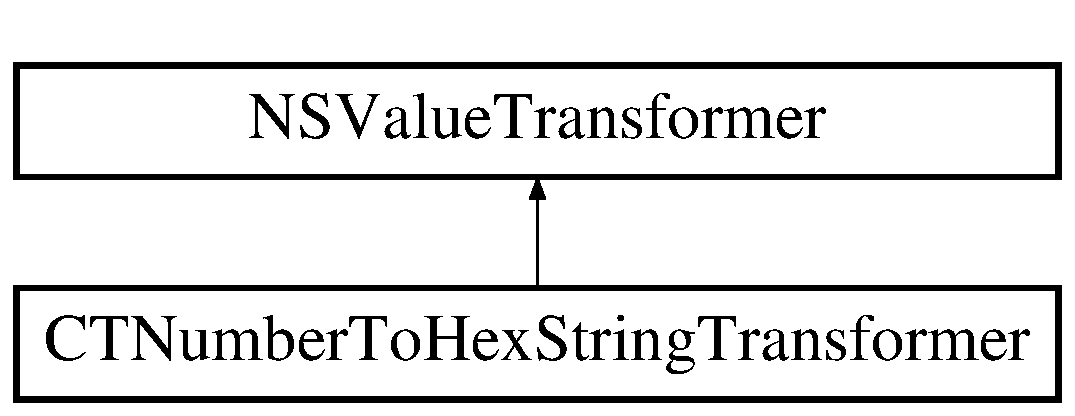
\includegraphics[height=2.000000cm]{interface_c_t_number_to_hex_string_transformer}
\end{center}
\end{figure}
\subsection*{Instance Methods}
\begin{DoxyCompactItemize}
\item 
(id) -\/ \hyperlink{interface_c_t_number_to_hex_string_transformer_ae4be8dcda663f1dbc6e12a8eb915ce34}{transformed\-Value\-:}
\begin{DoxyCompactList}\small\item\em Transforms a number into a hex string without the 0x, and no leading zeros. \end{DoxyCompactList}\item 
(id) -\/ \hyperlink{interface_c_t_number_to_hex_string_transformer_a00b54742110417a4a932da2a0277c7ad}{reverse\-Transformed\-Value\-:}
\begin{DoxyCompactList}\small\item\em Transforms a hex formatted N\-S\-String into an N\-S\-Number. \end{DoxyCompactList}\end{DoxyCompactItemize}
\subsection*{Class Methods}
\begin{DoxyCompactItemize}
\item 
(Class) + \hyperlink{interface_c_t_number_to_hex_string_transformer_a2ab81e9c3b57ee99a0d25c1f240ed59b}{transformed\-Value\-Class}
\item 
(B\-O\-O\-L) + \hyperlink{interface_c_t_number_to_hex_string_transformer_ab37052d53b55b38997a5c3c29f597134}{allows\-Reverse\-Transformation}
\end{DoxyCompactItemize}


\subsection{Method Documentation}
\hypertarget{interface_c_t_number_to_hex_string_transformer_ab37052d53b55b38997a5c3c29f597134}{\index{C\-T\-Number\-To\-Hex\-String\-Transformer@{C\-T\-Number\-To\-Hex\-String\-Transformer}!allows\-Reverse\-Transformation@{allows\-Reverse\-Transformation}}
\index{allows\-Reverse\-Transformation@{allows\-Reverse\-Transformation}!CTNumberToHexStringTransformer@{C\-T\-Number\-To\-Hex\-String\-Transformer}}
\subsubsection[{allows\-Reverse\-Transformation}]{\setlength{\rightskip}{0pt plus 5cm}+ (B\-O\-O\-L) allows\-Reverse\-Transformation 
\begin{DoxyParamCaption}
{}
\end{DoxyParamCaption}
}}\label{interface_c_t_number_to_hex_string_transformer_ab37052d53b55b38997a5c3c29f597134}
\hypertarget{interface_c_t_number_to_hex_string_transformer_a00b54742110417a4a932da2a0277c7ad}{\index{C\-T\-Number\-To\-Hex\-String\-Transformer@{C\-T\-Number\-To\-Hex\-String\-Transformer}!reverse\-Transformed\-Value\-:@{reverse\-Transformed\-Value\-:}}
\index{reverse\-Transformed\-Value\-:@{reverse\-Transformed\-Value\-:}!CTNumberToHexStringTransformer@{C\-T\-Number\-To\-Hex\-String\-Transformer}}
\subsubsection[{reverse\-Transformed\-Value\-:}]{\setlength{\rightskip}{0pt plus 5cm}-\/ (id) reverse\-Transformed\-Value\-: 
\begin{DoxyParamCaption}
\item[{(id)}]{value}
\end{DoxyParamCaption}
}}\label{interface_c_t_number_to_hex_string_transformer_a00b54742110417a4a932da2a0277c7ad}


Transforms a hex formatted N\-S\-String into an N\-S\-Number. 


\begin{DoxyParams}{Parameters}
{\em value} & a hex formatted N\-S\-String \\
\hline
\end{DoxyParams}
\begin{DoxyReturn}{Returns}
an N\-S\-Number 
\end{DoxyReturn}
\hypertarget{interface_c_t_number_to_hex_string_transformer_ae4be8dcda663f1dbc6e12a8eb915ce34}{\index{C\-T\-Number\-To\-Hex\-String\-Transformer@{C\-T\-Number\-To\-Hex\-String\-Transformer}!transformed\-Value\-:@{transformed\-Value\-:}}
\index{transformed\-Value\-:@{transformed\-Value\-:}!CTNumberToHexStringTransformer@{C\-T\-Number\-To\-Hex\-String\-Transformer}}
\subsubsection[{transformed\-Value\-:}]{\setlength{\rightskip}{0pt plus 5cm}-\/ (id) transformed\-Value\-: 
\begin{DoxyParamCaption}
\item[{(id)}]{value}
\end{DoxyParamCaption}
}}\label{interface_c_t_number_to_hex_string_transformer_ae4be8dcda663f1dbc6e12a8eb915ce34}


Transforms a number into a hex string without the 0x, and no leading zeros. 


\begin{DoxyParams}{Parameters}
{\em value,an} & number \\
\hline
\end{DoxyParams}
\begin{DoxyReturn}{Returns}
a hex formatted N\-S\-String 
\end{DoxyReturn}
\hypertarget{interface_c_t_number_to_hex_string_transformer_a2ab81e9c3b57ee99a0d25c1f240ed59b}{\index{C\-T\-Number\-To\-Hex\-String\-Transformer@{C\-T\-Number\-To\-Hex\-String\-Transformer}!transformed\-Value\-Class@{transformed\-Value\-Class}}
\index{transformed\-Value\-Class@{transformed\-Value\-Class}!CTNumberToHexStringTransformer@{C\-T\-Number\-To\-Hex\-String\-Transformer}}
\subsubsection[{transformed\-Value\-Class}]{\setlength{\rightskip}{0pt plus 5cm}+ (Class) transformed\-Value\-Class 
\begin{DoxyParamCaption}
{}
\end{DoxyParamCaption}
}}\label{interface_c_t_number_to_hex_string_transformer_a2ab81e9c3b57ee99a0d25c1f240ed59b}


The documentation for this class was generated from the following files\-:\begin{DoxyCompactItemize}
\item 
\hyperlink{_c_t_number_to_hex_string_transformer_8h}{C\-T\-Number\-To\-Hex\-String\-Transformer.\-h}\item 
\hyperlink{_c_t_number_to_hex_string_transformer_8m}{C\-T\-Number\-To\-Hex\-String\-Transformer.\-m}\end{DoxyCompactItemize}

\hypertarget{interface_c_t_number_to_string_formatter}{\section{C\-T\-Number\-To\-String\-Formatter Class Reference}
\label{interface_c_t_number_to_string_formatter}\index{C\-T\-Number\-To\-String\-Formatter@{C\-T\-Number\-To\-String\-Formatter}}
}


{\ttfamily \#import $<$C\-T\-Number\-To\-String\-Formatter.\-h$>$}

Inheritance diagram for C\-T\-Number\-To\-String\-Formatter\-:\begin{figure}[H]
\begin{center}
\leavevmode
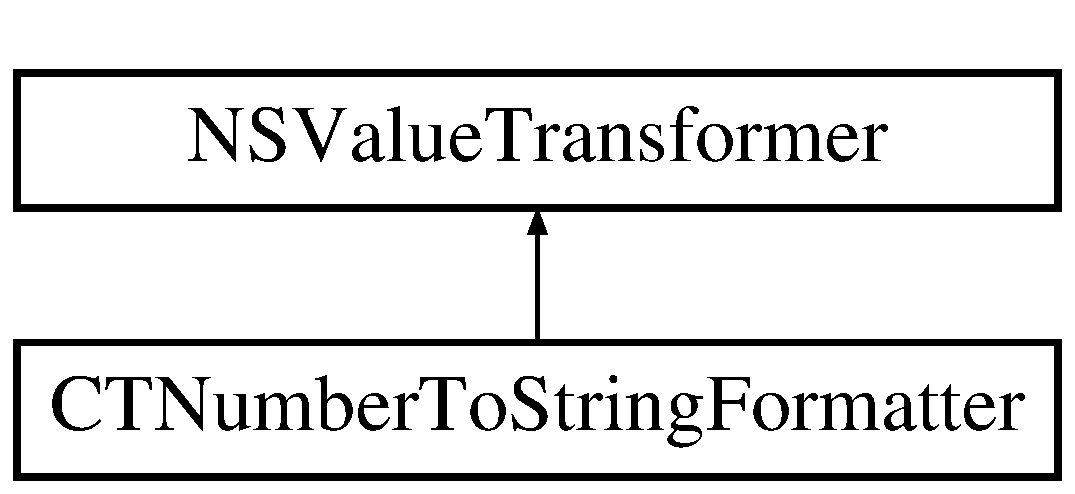
\includegraphics[height=2.000000cm]{interface_c_t_number_to_string_formatter}
\end{center}
\end{figure}
\subsection*{Instance Methods}
\begin{DoxyCompactItemize}
\item 
(id) -\/ \hyperlink{interface_c_t_number_to_string_formatter_a9d2e35f8862621f17a2a24006ab4e8b2}{transformed\-Value\-:}
\item 
(id) -\/ \hyperlink{interface_c_t_number_to_string_formatter_a2e18efc8fb4819f52cd335299229deb3}{reverse\-Transformed\-Value\-:}
\end{DoxyCompactItemize}
\subsection*{Class Methods}
\begin{DoxyCompactItemize}
\item 
(Class) + \hyperlink{interface_c_t_number_to_string_formatter_a2b8f857a79feecc7b108054619d641dc}{transformed\-Value\-Class}
\item 
(B\-O\-O\-L) + \hyperlink{interface_c_t_number_to_string_formatter_a59aa7be7f9270cf40a8e01bd21183520}{allows\-Reverse\-Transformation}
\end{DoxyCompactItemize}


\subsection{Method Documentation}
\hypertarget{interface_c_t_number_to_string_formatter_a59aa7be7f9270cf40a8e01bd21183520}{\index{C\-T\-Number\-To\-String\-Formatter@{C\-T\-Number\-To\-String\-Formatter}!allows\-Reverse\-Transformation@{allows\-Reverse\-Transformation}}
\index{allows\-Reverse\-Transformation@{allows\-Reverse\-Transformation}!CTNumberToStringFormatter@{C\-T\-Number\-To\-String\-Formatter}}
\subsubsection[{allows\-Reverse\-Transformation}]{\setlength{\rightskip}{0pt plus 5cm}+ (B\-O\-O\-L) allows\-Reverse\-Transformation 
\begin{DoxyParamCaption}
{}
\end{DoxyParamCaption}
}}\label{interface_c_t_number_to_string_formatter_a59aa7be7f9270cf40a8e01bd21183520}
\hypertarget{interface_c_t_number_to_string_formatter_a2e18efc8fb4819f52cd335299229deb3}{\index{C\-T\-Number\-To\-String\-Formatter@{C\-T\-Number\-To\-String\-Formatter}!reverse\-Transformed\-Value\-:@{reverse\-Transformed\-Value\-:}}
\index{reverse\-Transformed\-Value\-:@{reverse\-Transformed\-Value\-:}!CTNumberToStringFormatter@{C\-T\-Number\-To\-String\-Formatter}}
\subsubsection[{reverse\-Transformed\-Value\-:}]{\setlength{\rightskip}{0pt plus 5cm}-\/ (id) reverse\-Transformed\-Value\-: 
\begin{DoxyParamCaption}
\item[{(id)}]{value}
\end{DoxyParamCaption}
}}\label{interface_c_t_number_to_string_formatter_a2e18efc8fb4819f52cd335299229deb3}
\hypertarget{interface_c_t_number_to_string_formatter_a9d2e35f8862621f17a2a24006ab4e8b2}{\index{C\-T\-Number\-To\-String\-Formatter@{C\-T\-Number\-To\-String\-Formatter}!transformed\-Value\-:@{transformed\-Value\-:}}
\index{transformed\-Value\-:@{transformed\-Value\-:}!CTNumberToStringFormatter@{C\-T\-Number\-To\-String\-Formatter}}
\subsubsection[{transformed\-Value\-:}]{\setlength{\rightskip}{0pt plus 5cm}-\/ (id) transformed\-Value\-: 
\begin{DoxyParamCaption}
\item[{(id)}]{value}
\end{DoxyParamCaption}
}}\label{interface_c_t_number_to_string_formatter_a9d2e35f8862621f17a2a24006ab4e8b2}
\hypertarget{interface_c_t_number_to_string_formatter_a2b8f857a79feecc7b108054619d641dc}{\index{C\-T\-Number\-To\-String\-Formatter@{C\-T\-Number\-To\-String\-Formatter}!transformed\-Value\-Class@{transformed\-Value\-Class}}
\index{transformed\-Value\-Class@{transformed\-Value\-Class}!CTNumberToStringFormatter@{C\-T\-Number\-To\-String\-Formatter}}
\subsubsection[{transformed\-Value\-Class}]{\setlength{\rightskip}{0pt plus 5cm}+ (Class) transformed\-Value\-Class 
\begin{DoxyParamCaption}
{}
\end{DoxyParamCaption}
}}\label{interface_c_t_number_to_string_formatter_a2b8f857a79feecc7b108054619d641dc}


The documentation for this class was generated from the following files\-:\begin{DoxyCompactItemize}
\item 
\hyperlink{_c_t_number_to_string_formatter_8h}{C\-T\-Number\-To\-String\-Formatter.\-h}\item 
\hyperlink{_c_t_number_to_string_formatter_8m}{C\-T\-Number\-To\-String\-Formatter.\-m}\end{DoxyCompactItemize}

\chapter{File Documentation}
\hypertarget{_c_t_app_delegate_8h}{\section{C\-T\-App\-Delegate.\-h File Reference}
\label{_c_t_app_delegate_8h}\index{C\-T\-App\-Delegate.\-h@{C\-T\-App\-Delegate.\-h}}
}
{\ttfamily \#import $<$Cocoa/\-Cocoa.\-h$>$}\\*
{\ttfamily \#include \char`\"{}libusb.\-h\char`\"{}}\\*
\subsection*{Classes}
\begin{DoxyCompactItemize}
\item 
class \hyperlink{interface_c_t_app_delegate}{C\-T\-App\-Delegate}
\end{DoxyCompactItemize}
\subsection*{Macros}
\begin{DoxyCompactItemize}
\item 
\#define \hyperlink{_c_t_app_delegate_8h_ad26c49e2b9116716b7fa61e3d9030c39}{C\-T\-\_\-\-D\-I\-S\-P\-L\-A\-Y\-\_\-\-H\-E\-X}~0
\item 
\#define \hyperlink{_c_t_app_delegate_8h_a917b853c82a6172d39b8275fb7e80864}{C\-T\-\_\-\-D\-I\-S\-P\-L\-A\-Y\-\_\-\-P\-L\-A\-I\-N\-\_\-\-T\-E\-X\-T}~1
\end{DoxyCompactItemize}


\subsection{Macro Definition Documentation}
\hypertarget{_c_t_app_delegate_8h_ad26c49e2b9116716b7fa61e3d9030c39}{\index{C\-T\-App\-Delegate.\-h@{C\-T\-App\-Delegate.\-h}!C\-T\-\_\-\-D\-I\-S\-P\-L\-A\-Y\-\_\-\-H\-E\-X@{C\-T\-\_\-\-D\-I\-S\-P\-L\-A\-Y\-\_\-\-H\-E\-X}}
\index{C\-T\-\_\-\-D\-I\-S\-P\-L\-A\-Y\-\_\-\-H\-E\-X@{C\-T\-\_\-\-D\-I\-S\-P\-L\-A\-Y\-\_\-\-H\-E\-X}!CTAppDelegate.h@{C\-T\-App\-Delegate.\-h}}
\subsubsection[{C\-T\-\_\-\-D\-I\-S\-P\-L\-A\-Y\-\_\-\-H\-E\-X}]{\setlength{\rightskip}{0pt plus 5cm}\#define C\-T\-\_\-\-D\-I\-S\-P\-L\-A\-Y\-\_\-\-H\-E\-X~0}}\label{_c_t_app_delegate_8h_ad26c49e2b9116716b7fa61e3d9030c39}
\hypertarget{_c_t_app_delegate_8h_a917b853c82a6172d39b8275fb7e80864}{\index{C\-T\-App\-Delegate.\-h@{C\-T\-App\-Delegate.\-h}!C\-T\-\_\-\-D\-I\-S\-P\-L\-A\-Y\-\_\-\-P\-L\-A\-I\-N\-\_\-\-T\-E\-X\-T@{C\-T\-\_\-\-D\-I\-S\-P\-L\-A\-Y\-\_\-\-P\-L\-A\-I\-N\-\_\-\-T\-E\-X\-T}}
\index{C\-T\-\_\-\-D\-I\-S\-P\-L\-A\-Y\-\_\-\-P\-L\-A\-I\-N\-\_\-\-T\-E\-X\-T@{C\-T\-\_\-\-D\-I\-S\-P\-L\-A\-Y\-\_\-\-P\-L\-A\-I\-N\-\_\-\-T\-E\-X\-T}!CTAppDelegate.h@{C\-T\-App\-Delegate.\-h}}
\subsubsection[{C\-T\-\_\-\-D\-I\-S\-P\-L\-A\-Y\-\_\-\-P\-L\-A\-I\-N\-\_\-\-T\-E\-X\-T}]{\setlength{\rightskip}{0pt plus 5cm}\#define C\-T\-\_\-\-D\-I\-S\-P\-L\-A\-Y\-\_\-\-P\-L\-A\-I\-N\-\_\-\-T\-E\-X\-T~1}}\label{_c_t_app_delegate_8h_a917b853c82a6172d39b8275fb7e80864}

\hypertarget{_c_t_app_delegate_8m}{\section{C\-T\-App\-Delegate.\-m File Reference}
\label{_c_t_app_delegate_8m}\index{C\-T\-App\-Delegate.\-m@{C\-T\-App\-Delegate.\-m}}
}
{\ttfamily \#import \char`\"{}C\-T\-App\-Delegate.\-h\char`\"{}}\\*
{\ttfamily \#import \char`\"{}C\-T\-Number\-To\-Hex\-String\-Transformer.\-h\char`\"{}}\\*
{\ttfamily \#import \char`\"{}C\-T\-Number\-To\-String\-Formatter.\-h\char`\"{}}\\*
\subsection*{Variables}
\begin{DoxyCompactItemize}
\item 
N\-S\-String $\ast$const \hyperlink{_c_t_app_delegate_8m_a694671457e939c66551be38822e0b023}{C\-T\-Default\-\_\-\-Console\-Background\-Color\-\_\-\-Key} = @\char`\"{}console\-Background\-Color\char`\"{}
\item 
N\-S\-String $\ast$const \hyperlink{_c_t_app_delegate_8m_aa6e2fc00be91751da3ff400d21316aa9}{C\-T\-Default\-\_\-\-Console\-Error\-Text\-Color\-\_\-\-Key} = @\char`\"{}console\-Error\-Text\-Color\char`\"{}
\item 
N\-S\-String $\ast$const \hyperlink{_c_t_app_delegate_8m_ae513d8db59eee271b3421609ea6fdd75}{C\-T\-Default\-\_\-\-Console\-Data\-Text\-Color\-\_\-\-Key} = @\char`\"{}console\-Data\-Text\-Color\char`\"{}
\item 
N\-S\-String $\ast$const \hyperlink{_c_t_app_delegate_8m_a3ac89b6b7ee757f11dea83a64bdd450d}{C\-T\-Default\-\_\-\-Console\-Information\-Text\-Color\-\_\-\-Key} = @\char`\"{}console\-Information\-Text\-Color\char`\"{}
\item 
N\-S\-String $\ast$const \hyperlink{_c_t_app_delegate_8m_a0ba855f0e6b98ed4b8c8acaaa94e864c}{C\-T\-Default\-\_\-\-Display\-Hex\-Or\-Plain\-Text\-\_\-\-Key} = @\char`\"{}display\-Hex\-Or\-Plain\-Text\char`\"{}
\item 
N\-S\-String $\ast$const \hyperlink{_c_t_app_delegate_8m_a7cd3b9a765c756a77b39ee4313d20314}{C\-T\-Default\-\_\-\-V\-I\-D\-\_\-\-Key} = @\char`\"{}device\-V\-I\-D\char`\"{}
\item 
N\-S\-String $\ast$const \hyperlink{_c_t_app_delegate_8m_a586b869e25ae97c3cda189e0e2e899c0}{C\-T\-Default\-\_\-\-P\-I\-D\-\_\-\-Key} = @\char`\"{}device\-P\-I\-D\char`\"{}
\item 
N\-S\-String $\ast$const \hyperlink{_c_t_app_delegate_8m_a3ae3819c6f003d6612b24104cc133a26}{C\-T\-Default\-\_\-bm\-Request\-Type\-\_\-\-Key} = @\char`\"{}request\-Type\char`\"{}
\item 
N\-S\-String $\ast$const \hyperlink{_c_t_app_delegate_8m_a83a24d51d68e5cccf74a22b805509ab3}{C\-T\-Default\-\_\-bm\-Request\-Destination\-\_\-\-Key} = @\char`\"{}request\-Destination\char`\"{}
\item 
N\-S\-String $\ast$const \hyperlink{_c_t_app_delegate_8m_a57d37d709ca3ac59ceb9b4d6f5f5dec4}{C\-T\-Default\-\_\-b\-Request\-\_\-\-Key} = @\char`\"{}control\-Transfer\-Request\char`\"{}
\item 
N\-S\-String $\ast$const \hyperlink{_c_t_app_delegate_8m_a8758a0f0d361a4c3b18d6836d5a22741}{C\-T\-Default\-\_\-w\-Value\-\_\-\-Key} = @\char`\"{}control\-Transfer\-Value\char`\"{}
\item 
N\-S\-String $\ast$const \hyperlink{_c_t_app_delegate_8m_abc7a31d538c78541df73b156231b2ded}{C\-T\-Default\-\_\-w\-Index\-\_\-\-Key} = @\char`\"{}control\-Transfer\-Index\char`\"{}
\item 
N\-S\-String $\ast$const \hyperlink{_c_t_app_delegate_8m_a1c447a30d81ae588efa21ee53fa6b5fe}{C\-T\-Default\-\_\-w\-Length\-\_\-\-Key} = @\char`\"{}control\-Transfer\-Length\char`\"{}
\item 
N\-S\-String $\ast$const \hyperlink{_c_t_app_delegate_8m_a00fedd57b68287794c3f608b944c82ac}{C\-T\-Default\-\_\-endpoint\-\_\-\-Key} = @\char`\"{}bulk\-Transfer\-Endpoint\char`\"{}
\item 
N\-S\-String $\ast$const \hyperlink{_c_t_app_delegate_8m_abaea2d648d912fb248aa34a420dd0502}{C\-T\-Default\-\_\-bulk\-Transfer\-Length\-\_\-\-Key} = @\char`\"{}bulk\-Transfer\-Length\char`\"{}
\end{DoxyCompactItemize}


\subsection{Variable Documentation}
\hypertarget{_c_t_app_delegate_8m_a83a24d51d68e5cccf74a22b805509ab3}{\index{C\-T\-App\-Delegate.\-m@{C\-T\-App\-Delegate.\-m}!C\-T\-Default\-\_\-bm\-Request\-Destination\-\_\-\-Key@{C\-T\-Default\-\_\-bm\-Request\-Destination\-\_\-\-Key}}
\index{C\-T\-Default\-\_\-bm\-Request\-Destination\-\_\-\-Key@{C\-T\-Default\-\_\-bm\-Request\-Destination\-\_\-\-Key}!CTAppDelegate.m@{C\-T\-App\-Delegate.\-m}}
\subsubsection[{C\-T\-Default\-\_\-bm\-Request\-Destination\-\_\-\-Key}]{\setlength{\rightskip}{0pt plus 5cm}N\-S\-String$\ast$ const C\-T\-Default\-\_\-bm\-Request\-Destination\-\_\-\-Key = @\char`\"{}request\-Destination\char`\"{}}}\label{_c_t_app_delegate_8m_a83a24d51d68e5cccf74a22b805509ab3}
\hypertarget{_c_t_app_delegate_8m_a3ae3819c6f003d6612b24104cc133a26}{\index{C\-T\-App\-Delegate.\-m@{C\-T\-App\-Delegate.\-m}!C\-T\-Default\-\_\-bm\-Request\-Type\-\_\-\-Key@{C\-T\-Default\-\_\-bm\-Request\-Type\-\_\-\-Key}}
\index{C\-T\-Default\-\_\-bm\-Request\-Type\-\_\-\-Key@{C\-T\-Default\-\_\-bm\-Request\-Type\-\_\-\-Key}!CTAppDelegate.m@{C\-T\-App\-Delegate.\-m}}
\subsubsection[{C\-T\-Default\-\_\-bm\-Request\-Type\-\_\-\-Key}]{\setlength{\rightskip}{0pt plus 5cm}N\-S\-String$\ast$ const C\-T\-Default\-\_\-bm\-Request\-Type\-\_\-\-Key = @\char`\"{}request\-Type\char`\"{}}}\label{_c_t_app_delegate_8m_a3ae3819c6f003d6612b24104cc133a26}
\hypertarget{_c_t_app_delegate_8m_a57d37d709ca3ac59ceb9b4d6f5f5dec4}{\index{C\-T\-App\-Delegate.\-m@{C\-T\-App\-Delegate.\-m}!C\-T\-Default\-\_\-b\-Request\-\_\-\-Key@{C\-T\-Default\-\_\-b\-Request\-\_\-\-Key}}
\index{C\-T\-Default\-\_\-b\-Request\-\_\-\-Key@{C\-T\-Default\-\_\-b\-Request\-\_\-\-Key}!CTAppDelegate.m@{C\-T\-App\-Delegate.\-m}}
\subsubsection[{C\-T\-Default\-\_\-b\-Request\-\_\-\-Key}]{\setlength{\rightskip}{0pt plus 5cm}N\-S\-String$\ast$ const C\-T\-Default\-\_\-b\-Request\-\_\-\-Key = @\char`\"{}control\-Transfer\-Request\char`\"{}}}\label{_c_t_app_delegate_8m_a57d37d709ca3ac59ceb9b4d6f5f5dec4}
\hypertarget{_c_t_app_delegate_8m_abaea2d648d912fb248aa34a420dd0502}{\index{C\-T\-App\-Delegate.\-m@{C\-T\-App\-Delegate.\-m}!C\-T\-Default\-\_\-bulk\-Transfer\-Length\-\_\-\-Key@{C\-T\-Default\-\_\-bulk\-Transfer\-Length\-\_\-\-Key}}
\index{C\-T\-Default\-\_\-bulk\-Transfer\-Length\-\_\-\-Key@{C\-T\-Default\-\_\-bulk\-Transfer\-Length\-\_\-\-Key}!CTAppDelegate.m@{C\-T\-App\-Delegate.\-m}}
\subsubsection[{C\-T\-Default\-\_\-bulk\-Transfer\-Length\-\_\-\-Key}]{\setlength{\rightskip}{0pt plus 5cm}N\-S\-String$\ast$ const C\-T\-Default\-\_\-bulk\-Transfer\-Length\-\_\-\-Key = @\char`\"{}bulk\-Transfer\-Length\char`\"{}}}\label{_c_t_app_delegate_8m_abaea2d648d912fb248aa34a420dd0502}
\hypertarget{_c_t_app_delegate_8m_a694671457e939c66551be38822e0b023}{\index{C\-T\-App\-Delegate.\-m@{C\-T\-App\-Delegate.\-m}!C\-T\-Default\-\_\-\-Console\-Background\-Color\-\_\-\-Key@{C\-T\-Default\-\_\-\-Console\-Background\-Color\-\_\-\-Key}}
\index{C\-T\-Default\-\_\-\-Console\-Background\-Color\-\_\-\-Key@{C\-T\-Default\-\_\-\-Console\-Background\-Color\-\_\-\-Key}!CTAppDelegate.m@{C\-T\-App\-Delegate.\-m}}
\subsubsection[{C\-T\-Default\-\_\-\-Console\-Background\-Color\-\_\-\-Key}]{\setlength{\rightskip}{0pt plus 5cm}N\-S\-String$\ast$ const C\-T\-Default\-\_\-\-Console\-Background\-Color\-\_\-\-Key = @\char`\"{}console\-Background\-Color\char`\"{}}}\label{_c_t_app_delegate_8m_a694671457e939c66551be38822e0b023}
\hypertarget{_c_t_app_delegate_8m_ae513d8db59eee271b3421609ea6fdd75}{\index{C\-T\-App\-Delegate.\-m@{C\-T\-App\-Delegate.\-m}!C\-T\-Default\-\_\-\-Console\-Data\-Text\-Color\-\_\-\-Key@{C\-T\-Default\-\_\-\-Console\-Data\-Text\-Color\-\_\-\-Key}}
\index{C\-T\-Default\-\_\-\-Console\-Data\-Text\-Color\-\_\-\-Key@{C\-T\-Default\-\_\-\-Console\-Data\-Text\-Color\-\_\-\-Key}!CTAppDelegate.m@{C\-T\-App\-Delegate.\-m}}
\subsubsection[{C\-T\-Default\-\_\-\-Console\-Data\-Text\-Color\-\_\-\-Key}]{\setlength{\rightskip}{0pt plus 5cm}N\-S\-String$\ast$ const C\-T\-Default\-\_\-\-Console\-Data\-Text\-Color\-\_\-\-Key = @\char`\"{}console\-Data\-Text\-Color\char`\"{}}}\label{_c_t_app_delegate_8m_ae513d8db59eee271b3421609ea6fdd75}
\hypertarget{_c_t_app_delegate_8m_aa6e2fc00be91751da3ff400d21316aa9}{\index{C\-T\-App\-Delegate.\-m@{C\-T\-App\-Delegate.\-m}!C\-T\-Default\-\_\-\-Console\-Error\-Text\-Color\-\_\-\-Key@{C\-T\-Default\-\_\-\-Console\-Error\-Text\-Color\-\_\-\-Key}}
\index{C\-T\-Default\-\_\-\-Console\-Error\-Text\-Color\-\_\-\-Key@{C\-T\-Default\-\_\-\-Console\-Error\-Text\-Color\-\_\-\-Key}!CTAppDelegate.m@{C\-T\-App\-Delegate.\-m}}
\subsubsection[{C\-T\-Default\-\_\-\-Console\-Error\-Text\-Color\-\_\-\-Key}]{\setlength{\rightskip}{0pt plus 5cm}N\-S\-String$\ast$ const C\-T\-Default\-\_\-\-Console\-Error\-Text\-Color\-\_\-\-Key = @\char`\"{}console\-Error\-Text\-Color\char`\"{}}}\label{_c_t_app_delegate_8m_aa6e2fc00be91751da3ff400d21316aa9}
\hypertarget{_c_t_app_delegate_8m_a3ac89b6b7ee757f11dea83a64bdd450d}{\index{C\-T\-App\-Delegate.\-m@{C\-T\-App\-Delegate.\-m}!C\-T\-Default\-\_\-\-Console\-Information\-Text\-Color\-\_\-\-Key@{C\-T\-Default\-\_\-\-Console\-Information\-Text\-Color\-\_\-\-Key}}
\index{C\-T\-Default\-\_\-\-Console\-Information\-Text\-Color\-\_\-\-Key@{C\-T\-Default\-\_\-\-Console\-Information\-Text\-Color\-\_\-\-Key}!CTAppDelegate.m@{C\-T\-App\-Delegate.\-m}}
\subsubsection[{C\-T\-Default\-\_\-\-Console\-Information\-Text\-Color\-\_\-\-Key}]{\setlength{\rightskip}{0pt plus 5cm}N\-S\-String$\ast$ const C\-T\-Default\-\_\-\-Console\-Information\-Text\-Color\-\_\-\-Key = @\char`\"{}console\-Information\-Text\-Color\char`\"{}}}\label{_c_t_app_delegate_8m_a3ac89b6b7ee757f11dea83a64bdd450d}
\hypertarget{_c_t_app_delegate_8m_a0ba855f0e6b98ed4b8c8acaaa94e864c}{\index{C\-T\-App\-Delegate.\-m@{C\-T\-App\-Delegate.\-m}!C\-T\-Default\-\_\-\-Display\-Hex\-Or\-Plain\-Text\-\_\-\-Key@{C\-T\-Default\-\_\-\-Display\-Hex\-Or\-Plain\-Text\-\_\-\-Key}}
\index{C\-T\-Default\-\_\-\-Display\-Hex\-Or\-Plain\-Text\-\_\-\-Key@{C\-T\-Default\-\_\-\-Display\-Hex\-Or\-Plain\-Text\-\_\-\-Key}!CTAppDelegate.m@{C\-T\-App\-Delegate.\-m}}
\subsubsection[{C\-T\-Default\-\_\-\-Display\-Hex\-Or\-Plain\-Text\-\_\-\-Key}]{\setlength{\rightskip}{0pt plus 5cm}N\-S\-String$\ast$ const C\-T\-Default\-\_\-\-Display\-Hex\-Or\-Plain\-Text\-\_\-\-Key = @\char`\"{}display\-Hex\-Or\-Plain\-Text\char`\"{}}}\label{_c_t_app_delegate_8m_a0ba855f0e6b98ed4b8c8acaaa94e864c}
\hypertarget{_c_t_app_delegate_8m_a00fedd57b68287794c3f608b944c82ac}{\index{C\-T\-App\-Delegate.\-m@{C\-T\-App\-Delegate.\-m}!C\-T\-Default\-\_\-endpoint\-\_\-\-Key@{C\-T\-Default\-\_\-endpoint\-\_\-\-Key}}
\index{C\-T\-Default\-\_\-endpoint\-\_\-\-Key@{C\-T\-Default\-\_\-endpoint\-\_\-\-Key}!CTAppDelegate.m@{C\-T\-App\-Delegate.\-m}}
\subsubsection[{C\-T\-Default\-\_\-endpoint\-\_\-\-Key}]{\setlength{\rightskip}{0pt plus 5cm}N\-S\-String$\ast$ const C\-T\-Default\-\_\-endpoint\-\_\-\-Key = @\char`\"{}bulk\-Transfer\-Endpoint\char`\"{}}}\label{_c_t_app_delegate_8m_a00fedd57b68287794c3f608b944c82ac}
\hypertarget{_c_t_app_delegate_8m_a586b869e25ae97c3cda189e0e2e899c0}{\index{C\-T\-App\-Delegate.\-m@{C\-T\-App\-Delegate.\-m}!C\-T\-Default\-\_\-\-P\-I\-D\-\_\-\-Key@{C\-T\-Default\-\_\-\-P\-I\-D\-\_\-\-Key}}
\index{C\-T\-Default\-\_\-\-P\-I\-D\-\_\-\-Key@{C\-T\-Default\-\_\-\-P\-I\-D\-\_\-\-Key}!CTAppDelegate.m@{C\-T\-App\-Delegate.\-m}}
\subsubsection[{C\-T\-Default\-\_\-\-P\-I\-D\-\_\-\-Key}]{\setlength{\rightskip}{0pt plus 5cm}N\-S\-String$\ast$ const C\-T\-Default\-\_\-\-P\-I\-D\-\_\-\-Key = @\char`\"{}device\-P\-I\-D\char`\"{}}}\label{_c_t_app_delegate_8m_a586b869e25ae97c3cda189e0e2e899c0}
\hypertarget{_c_t_app_delegate_8m_a7cd3b9a765c756a77b39ee4313d20314}{\index{C\-T\-App\-Delegate.\-m@{C\-T\-App\-Delegate.\-m}!C\-T\-Default\-\_\-\-V\-I\-D\-\_\-\-Key@{C\-T\-Default\-\_\-\-V\-I\-D\-\_\-\-Key}}
\index{C\-T\-Default\-\_\-\-V\-I\-D\-\_\-\-Key@{C\-T\-Default\-\_\-\-V\-I\-D\-\_\-\-Key}!CTAppDelegate.m@{C\-T\-App\-Delegate.\-m}}
\subsubsection[{C\-T\-Default\-\_\-\-V\-I\-D\-\_\-\-Key}]{\setlength{\rightskip}{0pt plus 5cm}N\-S\-String$\ast$ const C\-T\-Default\-\_\-\-V\-I\-D\-\_\-\-Key = @\char`\"{}device\-V\-I\-D\char`\"{}}}\label{_c_t_app_delegate_8m_a7cd3b9a765c756a77b39ee4313d20314}
\hypertarget{_c_t_app_delegate_8m_abc7a31d538c78541df73b156231b2ded}{\index{C\-T\-App\-Delegate.\-m@{C\-T\-App\-Delegate.\-m}!C\-T\-Default\-\_\-w\-Index\-\_\-\-Key@{C\-T\-Default\-\_\-w\-Index\-\_\-\-Key}}
\index{C\-T\-Default\-\_\-w\-Index\-\_\-\-Key@{C\-T\-Default\-\_\-w\-Index\-\_\-\-Key}!CTAppDelegate.m@{C\-T\-App\-Delegate.\-m}}
\subsubsection[{C\-T\-Default\-\_\-w\-Index\-\_\-\-Key}]{\setlength{\rightskip}{0pt plus 5cm}N\-S\-String$\ast$ const C\-T\-Default\-\_\-w\-Index\-\_\-\-Key = @\char`\"{}control\-Transfer\-Index\char`\"{}}}\label{_c_t_app_delegate_8m_abc7a31d538c78541df73b156231b2ded}
\hypertarget{_c_t_app_delegate_8m_a1c447a30d81ae588efa21ee53fa6b5fe}{\index{C\-T\-App\-Delegate.\-m@{C\-T\-App\-Delegate.\-m}!C\-T\-Default\-\_\-w\-Length\-\_\-\-Key@{C\-T\-Default\-\_\-w\-Length\-\_\-\-Key}}
\index{C\-T\-Default\-\_\-w\-Length\-\_\-\-Key@{C\-T\-Default\-\_\-w\-Length\-\_\-\-Key}!CTAppDelegate.m@{C\-T\-App\-Delegate.\-m}}
\subsubsection[{C\-T\-Default\-\_\-w\-Length\-\_\-\-Key}]{\setlength{\rightskip}{0pt plus 5cm}N\-S\-String$\ast$ const C\-T\-Default\-\_\-w\-Length\-\_\-\-Key = @\char`\"{}control\-Transfer\-Length\char`\"{}}}\label{_c_t_app_delegate_8m_a1c447a30d81ae588efa21ee53fa6b5fe}
\hypertarget{_c_t_app_delegate_8m_a8758a0f0d361a4c3b18d6836d5a22741}{\index{C\-T\-App\-Delegate.\-m@{C\-T\-App\-Delegate.\-m}!C\-T\-Default\-\_\-w\-Value\-\_\-\-Key@{C\-T\-Default\-\_\-w\-Value\-\_\-\-Key}}
\index{C\-T\-Default\-\_\-w\-Value\-\_\-\-Key@{C\-T\-Default\-\_\-w\-Value\-\_\-\-Key}!CTAppDelegate.m@{C\-T\-App\-Delegate.\-m}}
\subsubsection[{C\-T\-Default\-\_\-w\-Value\-\_\-\-Key}]{\setlength{\rightskip}{0pt plus 5cm}N\-S\-String$\ast$ const C\-T\-Default\-\_\-w\-Value\-\_\-\-Key = @\char`\"{}control\-Transfer\-Value\char`\"{}}}\label{_c_t_app_delegate_8m_a8758a0f0d361a4c3b18d6836d5a22741}

\hypertarget{_c_t_number_to_hex_string_transformer_8h}{\section{C\-T\-Number\-To\-Hex\-String\-Transformer.\-h File Reference}
\label{_c_t_number_to_hex_string_transformer_8h}\index{C\-T\-Number\-To\-Hex\-String\-Transformer.\-h@{C\-T\-Number\-To\-Hex\-String\-Transformer.\-h}}
}
{\ttfamily \#import $<$Foundation/\-Foundation.\-h$>$}\\*
\subsection*{Classes}
\begin{DoxyCompactItemize}
\item 
class \hyperlink{interface_c_t_number_to_hex_string_transformer}{C\-T\-Number\-To\-Hex\-String\-Transformer}
\end{DoxyCompactItemize}

\hypertarget{_c_t_number_to_hex_string_transformer_8m}{\section{C\-T\-Number\-To\-Hex\-String\-Transformer.\-m File Reference}
\label{_c_t_number_to_hex_string_transformer_8m}\index{C\-T\-Number\-To\-Hex\-String\-Transformer.\-m@{C\-T\-Number\-To\-Hex\-String\-Transformer.\-m}}
}
{\ttfamily \#import \char`\"{}C\-T\-Number\-To\-Hex\-String\-Transformer.\-h\char`\"{}}\\*

\hypertarget{_c_t_number_to_string_formatter_8h}{\section{C\-T\-Number\-To\-String\-Formatter.\-h File Reference}
\label{_c_t_number_to_string_formatter_8h}\index{C\-T\-Number\-To\-String\-Formatter.\-h@{C\-T\-Number\-To\-String\-Formatter.\-h}}
}
{\ttfamily \#import $<$Foundation/\-Foundation.\-h$>$}\\*
\subsection*{Classes}
\begin{DoxyCompactItemize}
\item 
class \hyperlink{interface_c_t_number_to_string_formatter}{C\-T\-Number\-To\-String\-Formatter}
\end{DoxyCompactItemize}

\hypertarget{_c_t_number_to_string_formatter_8m}{\section{U\-S\-B Toolbox/\-C\-T\-Number\-To\-String\-Formatter.m File Reference}
\label{_c_t_number_to_string_formatter_8m}\index{U\-S\-B Toolbox/\-C\-T\-Number\-To\-String\-Formatter.\-m@{U\-S\-B Toolbox/\-C\-T\-Number\-To\-String\-Formatter.\-m}}
}
{\ttfamily \#import \char`\"{}C\-T\-Number\-To\-String\-Formatter.\-h\char`\"{}}\\*

\hypertarget{main_8m}{\section{main.\-m File Reference}
\label{main_8m}\index{main.\-m@{main.\-m}}
}
{\ttfamily \#import $<$Cocoa/\-Cocoa.\-h$>$}\\*
\subsection*{Functions}
\begin{DoxyCompactItemize}
\item 
int \hyperlink{main_8m_a0ddf1224851353fc92bfbff6f499fa97}{main} (int argc, char $\ast$argv\mbox{[}$\,$\mbox{]})
\end{DoxyCompactItemize}


\subsection{Function Documentation}
\hypertarget{main_8m_a0ddf1224851353fc92bfbff6f499fa97}{\index{main.\-m@{main.\-m}!main@{main}}
\index{main@{main}!main.m@{main.\-m}}
\subsubsection[{main}]{\setlength{\rightskip}{0pt plus 5cm}int main (
\begin{DoxyParamCaption}
\item[{int}]{argc, }
\item[{char $\ast$}]{argv\mbox{[}$\,$\mbox{]}}
\end{DoxyParamCaption}
)}}\label{main_8m_a0ddf1224851353fc92bfbff6f499fa97}

\addcontentsline{toc}{part}{Index}
\printindex
\end{document}
